\documentclass[a4paper]{article}
\usepackage{fontawesome}
\usepackage{tabularx}
\usepackage{fullpage,graphicx,tikz}

%\usepackage{doublespace}
%\setstretch{1.2}

\usepackage{ae}
\usepackage{CV}
\usepackage{xcolor}
\usepackage{hyperref}
\hypersetup{
	colorlinks=true,
      linkcolor=blue,
    urlcolor=blue}

\begin{document}

\pagestyle{empty}

%Ueberschrift
\begin{center}
\huge{\textsc{Curriculum Vitae}}
\vspace{\baselineskip}

\end{center}
\vspace{1.5\baselineskip}
\begin{minipage}{0.7\textwidth}
\Large{\textsc{MD.Al-Helal}}\\
\end{minipage}
\begin{minipage}{0.7\textwidth}
  \begin{tikzpicture}
    \clip(0,0)circle[radius=1.37cm,];
    \node{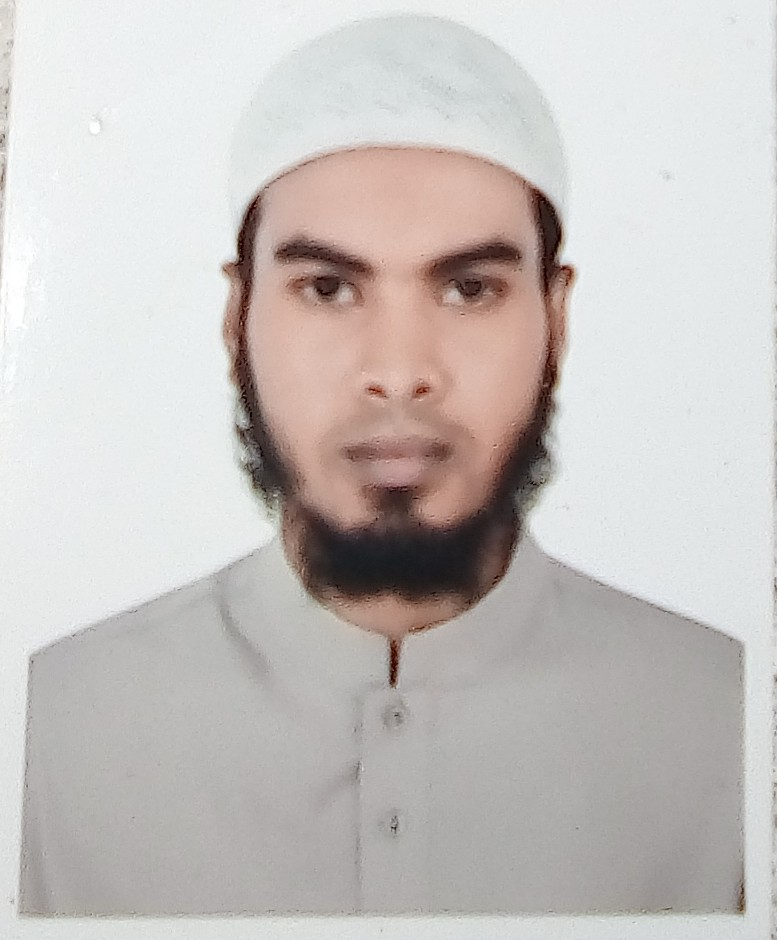
\includegraphics[scale=0.1]{myPhoto.jpg}};   
\end{tikzpicture}
\end{minipage}
\section{Address}
\noindent
\begin{minipage}{.7\textwidth}
  Room no-1406\\
  Shahid Sarafat Ali Building\\
  Dr. Muhammad Shahidullah Hall\\
  University of Dhaka\\
  Dhaka-1000\\
\end{minipage}
\begin{minipage}{.7\textwidth}
  \faPhone{} +8801515-611989\\
  \faEnvelopeO{}  \href{mailto:al2helal@gmail.com}{al2helal@gmail.com}\\
  \faEnvelopeO{}  \href{mailto:alhelal@ieee.org}{alhelal@ieee.org}\\
  \faGithub{}  \href{https://github.com/al2helal}{al2helal}\\
  \faLinkedin{}  \href{https://www.linkedin.com/in/mdalhelal/}{al2helal}\\
  \faStackOverflow{}  \href{https://stackoverflow.com/users/5697418/alhelal}{alhelal}
\end{minipage}

\section{Personal Details}
\begin{CV}
  \item[Gender] Male 
  \item[Father] Md.Akbar Ali
  \item[Mother] Most. Bilkis Begum
  \item[Date of birth] 2nd June, 1996
  \item[Permanent Address] Vill. Moyenpur, P.O. Kashimpur Hajigong-5460, Upa. Mithapukur, Dist. Rangpur
  \item[Nationality] Bangladeshi
  \item[Religion] Islam
  \end{CV}

\section{Career Objective}
\begin{CV}
\item To build up an efficient carrer in the computer science and engineering and thereby serve humanity.
  \end{CV}

\section{Working Experience}

\begin{CV}

\item[2018] Completed a project on making a e-commerce site(an online handicraft's store). I used PHP in back-end(server) and HTML, CSS, JavaScript, AJAX in front-end. I also used MySql in this project to build a MariaDB database.
\item[2017] Completed a project on making a suggestion provider text editor with IDE features. In this editor, user can edit and compile different programming languages's source code. The editor has a intelegence module that can help the user providing stackoverflow suggestion on his/her error of code.
%\item[2017] Completed a project on building a statistical predictive and recommendation model on universtity student's salary as tutor. I used R to complete this project.
\end{CV}


\section{Education}

\begin{CV}
\item[2015--current] University of Dhaka, Dhaka-1000.\\Continued  B.S in Computer Science \& Engineering. Currently in 4\textsuperscript{th} year.\\Obtained CGPA 3.33 (upto 3rd year)
\item[2014] Carmichael College, Rangpur.\\Passed H.S.C (Science Group) under Dinajpur Board in 2014.\\Obtained GPA 5.00 (without 4\textsuperscript{th} subject score) out of 5.00.
\item[2012] Moyenpur High School, Mithapukur, Rangpur.\\Passed S.S.C (Science Group) under Dinajpur Board in 2012.\\Obtained GPA 5.00 (without 4\textsuperscript{th} subject score) out of 5.00.
\end{CV}


%\section{Language Skills}
%\begin{table}[h] %\centering
%\begin{tabular}{p{2cm}>{}p{2.5cm}p{3cm}}
%Bangali  & native \\
%English  & 2nd language\\
%\end{tabular}
%\end{table}


%\section{Areas of Interest}
%\begin{CV}
%\item Machine learning, System programming, Making helpful shell script.
%\end{CV}


\section{Scholarship}

\begin{CV}
\item[2009] Obtained National Education Board Scholarship for good result in class 8.
\item[2014] Obtained National Education Board Scholarship for good result in H.S.C under Dinajpur Board.
\end{CV}

%\section{Technical Skills}
%\begin{table}[h]
%  \begin{tabular}{p{5cm}>{}p{6cm}}
%    Programming Languages  & C, Java, Sql, Mysql, HTML, R, Assembly\\
%    Tools & Oracle database, PhpMyadmin\\
%Version Control  & Git\\
%IDE & IntelliJ, Netbeans, Code Blocks\\
%Text Editor & Vim\\
%Operating System & Ubuntu, Fedora, Windows\\
%Typesetting & \LaTeX{}, Open office, Microsoft office\\
%\end{tabular}
%\end{table}

\section{Technical Skills}

\begin{CV}
\item[Languages]  Java, PHP, Python, C, Sql, Mysql, HTML, R, Assembly
\item[Tools] Oracle database, PhpMyadmin
\item[VCS] Git
\item[IDE] IntelliJ, Netbeans, Code Blocks
\item[Text Editor] Vim, VSCode
\item[OS] Ubuntu, Fedora, Kali Linux, Windows
\item[Typesetting] \LaTeX{}, Open office, Microsoft office
\end{CV}
\section{References}

\begin{table}[h]
\begin{tabular}{@{}lll@{}}
  \textbf{Dr. Md. Mustafizur Rahman}\\
  Professor \& Chairperson\\
Computer Science \& Engineering\\
University of Dhaka\\
\faPhone{} +8801927199301(Cell)\\
\faPhone (880)-2-9661900 Ext. 7433 (Office)\\
\faEnvelopeO{} \href{mailto:mustafiz@du.ac.bd}{mustafiz@du.ac.bd}\\
\faEnvelopeO{} \href{mailto:mustafiz1952@gmail.com}{mustafiz1952@gmail.com}\\
\faEnvelopeO{} \href{mailto:mustafiz1952@yahoo.com}{mustafiz1952@yahoo.com}\\
\end{tabular}
\end{table}

\noindent \today



\end{document}

%Tabellen
\begin{table}[htbp] \centering%
\begin{tabular}{lll}\hline\hline
1 & 2 & 3 \\ \hline
1 & \multicolumn{2}{c}{2} \\
\hline
\end{tabular}
\caption{Titel\label{Tabelle: Label}}
\end{table}

